% !TEX root = ../main.tex
\section{Forecast skill}
\label{sec:forecast}

Table~\ref{tab:eval} gives the rolling-origin scores of XGBoost by horizon. \textbf{The targets are met.} The relative WIS is below 1 at every horizon (\relWISHOne{} to \relWISHFour{}) and the 90\% coverage is inside the proposal's \targetCov{} band at every horizon (four weeks is close to the floor at \covNinetyHFour{}). The 50\% intervals are a little narrow (\covFiftyRange{}). The online conformal band reaches a similar coverage, a sign that the quantiles are not badly miscalibrated.

\begin{table}[htbp]
\centering
\caption{Forecast skill of XGBoost by horizon: WIS on case counts for XGBoost, XGBoost without the graph features and the seasonal-naive forecast; relative WIS against the naive forecast and against the no-graph model; empirical coverage.}
\label{tab:eval}
\footnotesize
\begin{tabular}{@{}l r r r r r r r r r@{}}
\toprule
horizon & $n$ & WIS & WIS no graph & WIS naive & rel.\ WIS & graph / no graph & cov.\ 50 & cov.\ 90 & cov.\ 90 conformal \\
\midrule
\tablerows{eval}
\bottomrule
\end{tabular}
\end{table}

\subsection{What carries the skill}

Table~\ref{tab:skill} compares the full model with its ablations, all scored on the same rows. XGBoost has a \relWISLowerPct{} lower WIS than the same week of the previous year. The graph adds nothing: it has \edgesEighteen{} links in the 2018 windows and \edgesNineteen{} in 2019, so leader signals are empty for most provinces. Rain, river, storm and flood features add nothing either. Two likely reasons, not tested: in a four-year panel rain moves with the season, so the season features already carry it, and any effect at lags beyond four weeks is outside this horizon. Figure~\ref{fig:fan} shows the forecasts for Cagayan, Ompong's landfall province.

\begin{table}[htbp]
\centering
\caption{Ablations: relative WIS of each comparison on the same rolling-origin rows.}
\label{tab:skill}
\small
\begin{tabularx}{\linewidth}{@{}l r L@{}}
\toprule
comparison & relative WIS & reading \\
\midrule
XGBoost against seasonal naive & \relWIS{} & \relWISLowerPct{} lower WIS than the same week last year \\
with against without graph leader features & \relWISGraph{} & no gain from the graph \\
with against without rain, river, storm and flood & \relWISEnv{} & \relWIS{} against \relWISNoEnv{} relative to seasonal naive \\
\bottomrule
\end{tabularx}
\end{table}

\begin{figure}[htbp]
\centering
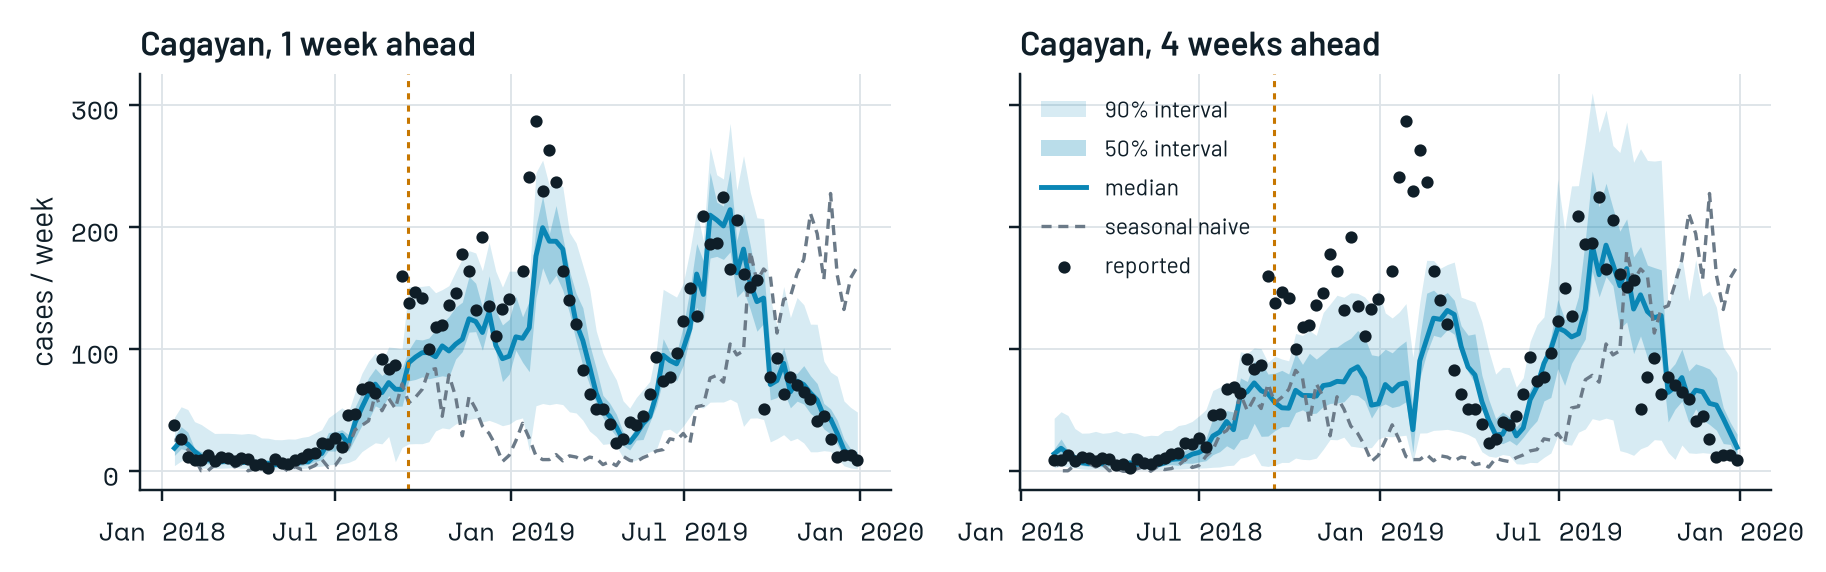
\includegraphics[width=\linewidth]{f05_fan}
\caption{Rolling-origin forecasts for Cagayan, one and four weeks ahead; the dashed line marks Ompong's landfall.}
\label{fig:fan}
\end{figure}

\subsection{Model comparison}
\label{sec:models}

Every model is scored on the same \nCommon{} rolling-origin rows (2018--2019, horizons \horizons{}, WIS on case counts). Table~\ref{tab:models} gives the relative WIS against the seasonal naive (below 1 is better) and against XGBoost; Figure~\ref{fig:wis} shows the same with the coverage by horizon.

\begin{table}[htbp]
\centering
\caption{Model comparison on the same rows, ordered by relative WIS. Bold: the best model on the mean and the operational model.}
\label{tab:models}
\footnotesize
\begin{tabularx}{\linewidth}{@{}L l r r r r r r r r@{}}
\toprule
model & kind & mean WIS & median WIS & rel.\ 1~wk & rel.\ 4~wk & rel.\ WIS & vs XGB & cov.\ 50 & cov.\ 90 \\
\midrule
\tablerows{models}
\bottomrule
\end{tabularx}
\end{table}

\begin{figure}[htbp]
\centering
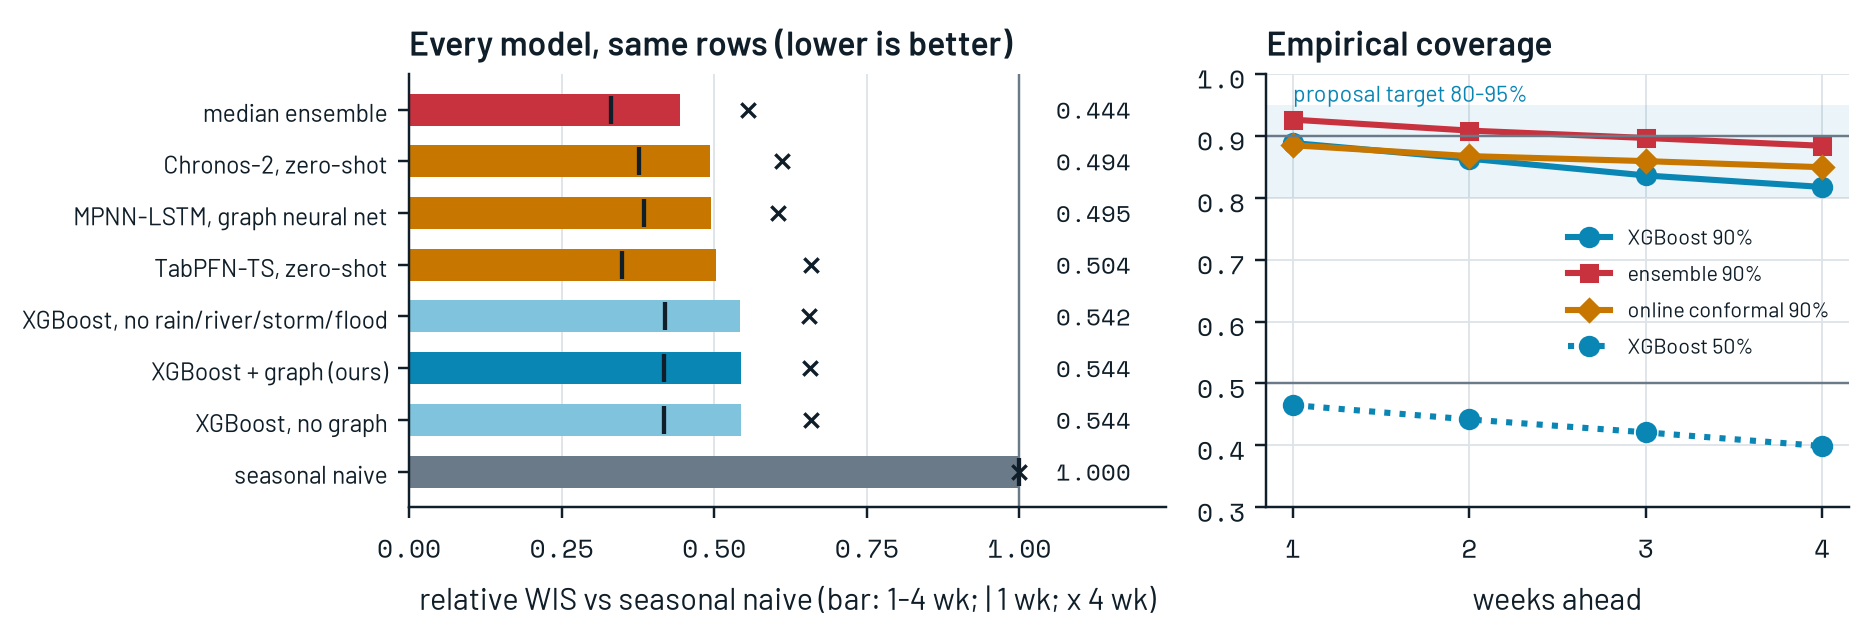
\includegraphics[width=\linewidth]{f03_wis}
\caption{Left: relative WIS of every model over one to four weeks (ticks: one and four weeks). Right: coverage against the nominal lines and the proposal's band.}
\label{fig:wis}
\end{figure}

\begin{itemize}
\item \textbf{Mean against median.} Every benchmark beats XGBoost on mean WIS, and the ensemble is best. On the median XGBoost is best (\mwXGB{} cases against \mwBenchRange{}; ensemble \mwEns{}). Split at the 90th percentile of weekly cases (\splitThr{}): below it the benchmarks' mean WIS is \splitLoRange{} times XGBoost's, above it \splitHiRange{} times. The better means come from the large-count epidemic weeks; the ensemble (\ensSplitLo{} below, \ensSplitHi{} above) gains in both.
\item \textbf{Chronos-2} as first specified, on $\log(1 + \text{incidence})$, collapsed on one-week reporting spikes (relative WIS \chronosLogRelWIS{}). The headline run uses the incidence scale with past-only covariates; it was chosen \emph{after} seeing that failure. Without covariates it scores \chronosNoCovRelWIS{}, so the covariates do not help.
\item \textbf{TabPFN-TS} runs univariate (it ignores past-only covariates) with the ungated TabPFN v2 regressor; the default v3.5 weights need a login and licence and were not used. A lagged-covariate variant scores \tabpfnLagCovRelWIS{}.
\item \textbf{MPNN-LSTM} uses border adjacency (\mpnnBorderEdges{} edges) plus ferry routes (\mpnnFerryEdges{} more, a 2024--2026 proxy); with no graph it scores \mpnnNoneRelWIS{}, the same within seed noise, in line with the sparse lead-lag graph.
\item \textbf{Where it is used.} The benchmarks and the ensemble exist only at the rolling-origin weeks of 2018--2019. Storm scenarios, shifted tracks, 2020 and the storm catalogue use XGBoost with calibrated $R$, because the zero-shot models take no storm-track input.
\end{itemize}
